\documentclass[paper=a4, fontsize=11pt, BCOR=13mm, DIV=13, headinclude, toc=index, toc=bibliography, english, twoside, parskip]{scrreprt}
% Die verwendete Dokumentenklasse ist scrreprt. Die verwendeten Optionen sind:
%
% paper=a4              Papier ist a4.
% fontsize=11pt         Schrifgröße ist 11.
% DIV=13                Das Papier wird in d viele Spalten und d' viele Zeilen eingeteilt. Die Werte werden aus DIV berechnet.
% BCOR=1cm              Definiert den Patz, der auf der Innenseite beim Binden verloren geht.
% headinclude           sorgt dafür, dass genug Platz für die Header vorhanden ist.
% toc=index             legt im Inhaltsverzeichnis einen Eintrag für das Stichwortverzeichnis an.
% toc=bibliography      legt im Inhaltsverzeichnis einen Eintrag für das Literaturverzeichnis an.
% english               englische Worte wie "Chapter" und "References".
% twoside               Beidseitiges Dokument, wie in einem Buch.


%If you don't want this fancyheaders comment out lines 17 to 24
% Fancyheader
\usepackage{fancyhdr}                   % Wie der Name schon sagt, um fancy Header zu generieren.
\pagestyle{fancy}                       % Fancy Header sollen angezeigt werden
\renewcommand{\sectionmark}[1]{\markright{\thesection.\ #1}{}}    % Verhindert dass rightmark ausschließlich Grußbuchstaben benutzt
\fancyhead[LE,RO]{\rightmark}           % Links bei geraden und rechts bei ungeraden Seitenzahlen soll der Name der Section stehen.
\fancyhead[LO,RE]{}                     % Links bei ungeraden und rechts bei geraden Seitenzahlen soll nichts stehen.
\fancyfoot[C]{}                         % Keine mittigen Seitenzahlen
\fancyfoot[LE,RO]{\thepage}             % Seitenzahlen unten in die jeweilige äußere Ecke





\setcounter{secnumdepth}{3}     % Nummerierungstiefe (chapter, section, subsection, ...).
\setcounter{tocdepth}{3}        % Nummerierungstiefe im Inhaltsverzeichn is.

\usepackage[linesnumbered,ruled,vlined]{algorithm2e}    % Algorithmen setzen.
\newcommand{\SkipBeforeAndAfter}{\vspace{8mm}}
%\SetAlgoSkip{SkipBeforeAndAfter}
%\SetAlgoSkip{bigskip} 
%\usepackage{algorithm}
%\usepackage{algpseudocodex}
%\algrenewcommand\algorithmicrequire{\textbf{Input:}}
%\algrenewcommand\algorithmicensure{\textbf{Output:}}
%\algnewcommand{\LeftComment}[1]{\Statex \(\triangleright\) #1}
\usepackage{amsmath,amssymb,amsthm,amsfonts,amsbsy,latexsym}    % "Notwendige" AMS-Math Pakete.
\usepackage{array}                      % Bessere Tabellen.
\renewcommand{\arraystretch}{1.15}      % Tabellen bekommen ein wenig mehr Platz.
\usepackage{bbm}                        % Dicke 1.
\usepackage[utf8]{inputenc}             % utf8 als Eingabeformat. should be loaded before biblatex
\usepackage[backend=biber, style=alphabetic, giveninits=true]{biblatex}  % Gute Erweiterung zu bibtex, Wird für Referenzen benutzt.
\bibliography{masterthesis_your_name_bibliography}   % Die verwendeten Referenzen (.bib-Datei)
\usepackage[hypcap]{caption}            % Damit Hyperrefs bei der figure-Umgebung auf die Figure zeigt statt auf die Caption.
\captionsetup{font=footnotesize} 
\usepackage{hyperref}
\usepackage{cleveref}
\usepackage{datetime}                   % Um \today einzustellen.
\newdateformat{mydate}{\THEDAY{}th \monthname{} \THEYEAR{}}
\usepackage{diagbox}                    % Diagonale in Tabellen.
\usepackage{enumitem}                   % Zum Ändern der Nummerierungsumgenung 'enumerate'
\setlist[enumerate,1]{label=(\roman*)}  % Aufzählungen sind vom Typ 'Klammer auf; kleine römische Zahl; Klammer zu'
\usepackage[T1]{fontenc}                % Bessere Schrift
\usepackage{ifthen}                     % Zum checken ob Parameter leer sind.
\usepackage{lmodern}                    % Bessere Schrift
\usepackage{listings}                   % Code Listings.
\usepackage{mathtools}                  % Subscript unter Summen behandeln. Der Befehl lautet \mathclap.
\usepackage{makeidx}                    % Stichwortverzeichnis.
\makeindex                              % Stichwortverzeichnis erstellen.
\renewcommand{\indexname}{Index}        % Name des Index definieren.
\usepackage{multirow}                   % In Tabellen mehrere Zeilen zu einer machen.
%\usepackage[parfill]{parskip}
\usepackage{rotating}                   % Um Figures zu drehen.
\usepackage{scrhack}                    % Verbessert die Zusammenarbeit von KOMA mit anderen Paketen (z.B, listing).
\usepackage{stackrel}                   % Symbole übereinander stapeln.
\usepackage[dvipsnames]{xcolor}         % Gefärbter Text und so.
\usepackage{tikz}                       % Graphen und kommutative Diagramme. Muss nach xcolor eingebunden werden.
\usepackage{tikz-cd}                    % Kommutative Diagramme.
\usepackage{transparent}                % Braucht mal manchmal für inkscape bilder.
\usetikzlibrary{patterns}               % Zu malen von schraffierten Flächen.

\graphicspath{{pictures/}}              % Pfad in dem die mit Inkscape erstellen Bilder liegen (relativ zum Hauptverzeichnis).

% Workaround, damit keine unnötigen Leerzeichen entstehen.
\let\oldindexdefn\index
\renewcommand*{\index}[1]{\oldindexdefn{#1}\ignorespaces}
\let\oldlabeldefn\label
\renewcommand*{\label}[1]{\oldlabeldefn{#1}\ignorespaces}

% Workaround, Linebreak nach ldots erlaubt.
\newcommand{\origldots}{}
\let\origldots\ldots
\renewcommand{\ldots}{\allowbreak\origldots}


% Symbolverzeichnis
\usepackage[intoc, english]{nomencl}     % Symbolverzeichnis.
% intoc                 die Symbolliste in das Inhaltsverzeichnis aufnehmen.
% english               englische Worte wie "Seite".
\renewcommand{\nomname}{Symbol Index}   % Definiert die Überschrift des Symbolverzeichnises.
\renewcommand{\nomlabelwidth}{80pt}     % Platz der einem Symbol gegönnt wird.
\newcommand{\symbolindex}[4][]{{\nomenclature[#1]{#2}{#3\ifthenelse{\equal{#4}{}}{}{ -- #4}\nomnorefpage}}\ignorespaces}    % Verbesserte Version von "\nomenclature". Erzeugt Symbol Beschreibung - Referenz.
\renewcommand*{\nompreamble}{\markright{\nomname}}    % Workaround: Fancyhdr schreibt im Symbolverzeichnis sonst den Namen des leztztes Kapitels.
\makenomenclature                       % Symbolverzeichnis erstellen.

% Anklickbare Referenzen (letztes eingebundenes Paket)
\usepackage{hyperref}                   % Referenzen innerhalb des Dokuments anklickbar machen. Achtung: Muss das letzte Paket im Präambel sein.
\hypersetup{                            % Optionen von hyperref Einstellen.
    colorlinks=true,                    % gefärbte Links an Stelle von Boxen.
    linkcolor=black,                     % Farbe interner Links.
    citecolor=black,                     % Farbe von Referenzen.
    urlcolor=black                       % Farbe von Internetlinks.
}

\usepackage{BA_Titelseite}


%Namen des Verfassers der Arbeit
\author{Solveig Tr\"ankner}
%Geburtsdatum des Verfassers
\geburtsdatum{12. März 2002}
%Gebortsort des Verfassers
\geburtsort{Wiesbaden, Hessen}
%Datum der Abgabe der Arbeit
%\date{\today}
\date{21. M\"arz 2025}

%Name des Betreuers
% z.B.: Prof. Dr. Peter Koepke
\betreuer{Betreuer: Prof. Dr. Jochen Garcke}
%Name des Zweitgutachters
\zweitgutachter{Zweitgutachterin: offen}
%Name des Instituts an dem der Betreuer der Arbeit tätig ist.
%z.B.: Mathematisches Institut
%\institut{Institut XYZ}
%\institut{Mathematisches Institut}
%\institut{Institut f\"ur Angewandte Mathematik}
\institut{Institut f\"ur Numerische Simulation}
%\institut{Forschungsinstitut f\"ur Diskrete Mathematik}
%Titel der Bachelorarbeit
\title{Data Visualization with t-SNE in Theory and Practice}
%Do not change!
\ausarbeitungstyp{Bachelorarbeit Mathematik}


%       Theoreme
\theoremstyle{definition}               % Name: dick            Text: normal.
%\newtheorem{defi}{Definition}[section]  % Der Zähler ist defi = Sectionzähler.1 . Sectionzähler soll bei Benutzung von defi nicht erhöht werden.
\newtheorem{defi}{Definition}[chapter]
\newtheorem*{defi*}{Definition}
\newtheorem{example}[defi]{Example}
\newtheorem{notation}[defi]{Notation}
\newtheorem{rem}[defi]{Remark}
\AtBeginEnvironment{rem}{%
  \pushQED{\qed}\renewcommand{\qedsymbol}{$\triangle$}%
}
\AtEndEnvironment{rem}{\popQED\endexample}
\newtheorem{defcor}[defi]{Definition/Corollary}
\newtheorem{defprop}[defi]{Definition/Proposition}
\newtheorem{defthm}[defi]{Definition/Theorem}

\newtheorem*{idea}{Idea}
\newtheorem*{question}{Question}
\newtheorem*{obs}{Observation}
\newtheorem*{prob}{Problem}
\newtheorem*{but}{But}
\newtheorem*{reci}{Recipe}

\theoremstyle{plain}
\newtheorem*{conj}{Conjecture}
\newtheorem{cor}[defi]{Corollary}
\newtheorem{lem}[defi]{Lemma}
\newtheorem{prop}[defi]{Proposition}
\newtheorem*{prop*}{Proposition}
\newtheorem{thm}[defi]{Theorem}
\newtheorem*{thm*}{Theorem}


%       Makros
\newcommand{\bA}{\mathbb{A}}
\newcommand{\bB}{\mathbb{B}}
\newcommand{\bC}{\mathbb{C}}
\newcommand{\bD}{\mathbb{D}}
\newcommand{\bE}{\mathbb{E}}
\newcommand{\bF}{\mathbb{F}}
\newcommand{\bG}{\mathbb{G}}
\newcommand{\bH}{\mathbb{H}}
\newcommand{\bI}{\mathbb{I}}
\newcommand{\bJ}{\mathbb{J}}
\newcommand{\bK}{\mathbb{K}}
\newcommand{\bL}{\mathbb{L}}
\newcommand{\bM}{\mathbb{M}}
\newcommand{\bN}{\mathbb{N}}
\newcommand{\bO}{\mathbb{O}}
\newcommand{\bP}{\mathbb{P}}
\newcommand{\bQ}{\mathbb{Q}}
\newcommand{\bR}{\mathbb{R}}
\newcommand{\bS}{\mathbb{S}}
\newcommand{\bT}{\mathbb{T}}
\newcommand{\bU}{\mathbb{U}}
\newcommand{\bV}{\mathbb{V}}
\newcommand{\bW}{\mathbb{W}}
\newcommand{\bX}{\mathbb{X}}
\newcommand{\bY}{\mathbb{Y}}
\newcommand{\bZ}{\mathbb{Z}}

\newcommand{\bfn}{\mathbf{n}}
\newcommand{\bfx}{\mathbf{x}}
\newcommand{\bfy}{\mathbf{y}}
\newcommand{\bs}[1]{{\boldsymbol#1}}

%\newcommand{\dd}{\mathrm{d}} 
\newcommand{\dd}{\operatorname{d}\!}
\newcommand{\inv}{^{-1}}
\newcommand*{\hm}{^H}
\newcommand*{\tp}{^T}

\newcommand\cconj[1]{\mathop{\overline{#1}}}
\newcommand\closure[1]{\overline{#1}}

\DeclareMathOperator{\spn}{span}
\DeclareMathOperator{\intr}{\text{int}}
\DeclareMathOperator{\rk}{\text{rank}}
\DeclareMathOperator{\diag}{diag}
\DeclareMathOperator{\Ima}{\text{Im}}

%\DeclarePairedDelimiter{\abs}{\lvert}{\rvert}
%\DeclarePairedDelimiter{\norm}{\lVert}{\rVert}

\newcommand\comment[1]{\textcolor{magenta}{\emph{#1}}}


\begin{document}
% Titelseite
\maketitle              % Titelseite ausgeben

\begin{abstract}
    \textbf{Abstract (English)}

    We propose a numerical method to compute stochastic quantities of interest of the Dirichlet Laplacian eigenvalue problem on randomly shaped domains.
    Our approach aims to exploit the stochastic properties of eigenspaces, which, contrary to individual eigenpairs, remain meaningful for eigenvalues of higher multiplicity.
    Using a representation formula, one can obtain an equivalent nonlinear eigenvalue problem for the single layer boundary integral operator, which we discretize by means of a Galerkin boundary element method.
    We employ a contour integral method to solve the discretization by reducing it to a linear eigenvalue problem that inherits its structure. This means that it has the same eigenvalues and multiplicities, and it is possible to obtain approximations of the corresponding eigenfunctions.
    We present a multilevel Monte Carlo quadrature method with a meaningful sampling strategy where we relate the eigenspaces to each other using invariant reference spaces, which allows for a satisfactory computation of expectations of eigenvalues.
    A numerical experiment that validates our proposed approach is given.
    %In this thesis we consider stochastic nonlinear operator-valued eigenvalue problems, in particular the 


    \vspace{2em}
    \textbf{Abstract (German)}

    Wir stellen eine numerische Methode zur Berechnung stochastischer Gr\"{o}\ss en des Dirichlet-Laplaceschen Eigenwertproblems auf zuf\"{a}llig geformten Gebieten vor.
    Unser Ansatz nutzt die stochastischen Eigenschaften der Eigenr\"{a}ume aus, die, im Gegensatz zu den individuellen Eigenpaaren, auch bei vielfachen Eigenwerten bedeutsam bleiben.
    %Im Rahmen der Eigenwertprobleme f\"{u}r holomorphe Fredholm-Operator-wertige Funktionen, kombinieren wir Wissen zur Galerkin-Randelement-Methode für dieses Problem mit einer Kontur-Integral-Methode zur L\"{o}sung nichtlinearer Eigenwertprobleme, um unser Problem auf ein lineares Eigenwertproblem zu reduzieren, das die Struktur des urspr\"{u}nglichen Problems beibehält, das hei\ss t, es hat die gleichen Eigenwerte und Vielfachheiten und es ist möglich, Approximationen der entsprechenden Eigenfunktionen zu erhalten.
    Mithilfe einer Darstellungsformel kann man das Problem äquivalent als ein nichtlineares Eigenwertproblem für den entsprechenden Einfachschichtoperator formulieren. Dieses diskretisieren wir über eine Galerkin-Randelement-Methode.
    Zum Lösen des nichtlinearen Eigenwertproblems verwenden wir eine Kontur-Integral-Methode, die die Diskretisierung auf ein lineares Eigenwertproblem reduziert, das die Struktur des urspr\"{u}nglichen Problems beibehält.
    Das hei\ss t, dass es die gleichen Eigenwerte und Vielfachheiten hat und es möglich ist, Approximationen der entsprechenden Eigenfunktionen zu erhalten.
    Wir stellen eine Multilevel-Monte-Carlo-Simulation vor, um Erwartungswerte der Eigenwerte zu berechnen.
    Dabei verwenden wir eine sinnvolle Sampling-Strategie, bei der wir Eigenräume über gemeinsame Referenzräume miteinander in Verbindung setzen.
    Wir präsentieren numerische Resultate, die unsere Vorgehensweise unterstützen.

\end{abstract}
\cleardoublepage

\setcounter{page}{5}    % Die Titelseite und die darauffolgende leere Seite sollen gefälligst Seite 1 und 2 sein.
\tableofcontents        % Inhaltsverzeichnis ausgeben
%\listofalgorithms

% Einleitung
\cleardoublepage        % Kapitel immer rechts beginnen
\chapter{Introduction}

In our modern world, we are confronted with an ever-growing amount of data. 
Statista estimated the amount of data created, captured, copied and consumed worldwide in 2023 to be a staggering 123 zetabytes, up from two zetabytes in the year 2010 \cite{Statista}.
As the amount of data grows, it also becomes much harder to analyze. 
What makes data analysis even harder is when the dimensionality of the data grows. 
This is increasingly the case in areas such as computer vision, where images are represented by hundreds if not thousands of pixels and natural language processing, where words are transformed into high-dimensional vectors, for example via word2vec \cite{word2vec}.
With such high-dimensional data, it is impossible to just \enquote{quickly take a look at it}. 
Traditional data visualization methods, such as boxplots or standard scatterplots are unable to visualize more than three dimensions effectively. 

\textcolor{red}{A sentence I like from \cite{vdMaa14}: \enquote{Visual exploration is an essential component of data analysis, as it allows for the development of intuitions and hypotheses for the processes that generated the data.}} 

To address this problem, new methods for visualizing high-dimensional data have been proposed. 
The t-Stochastic Neighbour Embedding (t-SNE) algorithm was first developed in 2008 \cite{vdMaa08} and built on prior work on Stochastic Neighbour Embeddings \cite{Hinton02}. 
It has gained a lot of popularity in bioinformatics (cite other biology papers), especially in  single-cell transcriptomics (cite Tasic, macosko, Cao). 
It is also used in cancer research (cite cancer papers here). 
But the use of t-SNE extends to very diverse areas, from finance (cite finance paper here) to computer security and natural language processing. 

\textcolor{red}{maybe mention that t-SNE is not only used for visualization, but can for example also be used as preprocessing before applying a clustering algorithm}

This widespread adoption of the algorithm can be explained by its effectiveness at what it sets out to do. Unlike other dimensionality algorithms, t-SNE was developed with the aim of 2D and 3D visualizations of data in mind. 
By focusing on retaining local structures in the low-dimensional embedding, t-SNE often successfully reveals clusters present in the data. 
Since t-SNE addresses the so-called crowding problem (see below), the embeddings it produces are often visually appealing.  

On a high-level, t-SNE works as follows: from the given points, we calculate a probability distribution that measures pairwise similarities between the data points. 
For the low-dimensional embedding, we start with some data points in 2D or 3D and also construct a distribution of pairwise similarities between these points. 
The t-SNE algorithm then iteratively modifies the location of the low-dimensional datapoints such that the difference between these two distributions, as measured by the Kullback-Leibler divergence, is minimized. 
A different way to understand the algorithm is through the lense of dynamical systems, as described by \cite{LinStei22}. 
One can think of every datapoint as a physical particle which experiences two types of forces: an attractive force to its nearest neighbors in the high-dimensional space and a repulsive force towards all other particles \cite{KoBe19SingleCell}. 

Although t-SNE often works well, there are also some drawbacks to the method. 
Firstly, t-SNE requires the practitioner to make choices regarding the values of some hyperparameters. 
While common libraries \cite{openTSNE, sklearn_api} come with standard parameter settings, it is not uncommon in practice to run the algorithm multiple times with different parameters. 
In particular, the impact of the perplexity parameter, which determines the number of neighbors we consider when constructing the high-dimensional probability distribution, has been studied extensively (\textcolor{red}{include all perplexity citations here}). 

As pointed out by \cite{KoBe19SingleCell}, the perplexity parameter is often perceived as being the only parameter that needs tuning. 
But \enquote{under the hood [...] there are also
various optimisation parameters (such as the learning rate, the
number of iterations, early exaggeration factor, etc.)} \cite{KoBe19SingleCell}, which have been shown to also have a great impact on the quality of the embedding. 
This is problematic, since it is impractical to tune every single parameter and different parameter choices can lead to very different results, making it hard to interpret the results. 
Furthermore, the exact impact of each of these parameters on the embedding is not entirely clear, especially to practioners who are not experts in the field of dimensionality reduction. 


Secondly, there is still a lack of understanding of the internal workings of the algorithm. 
After t-SNE became popular, there also began to appear papers investigating it from a theoretical viewpoint. 
For example, several clustering guarantees have been proposed and the behaviour of t-SNE as the number of datapoints goes to infinity has been studied (\textcolor{red}{add citation here}). 
But difficulties formulating theorems that are applicable to real-world datasets persist, with papers making a number of assumptions that are sometimes disconnected from practice. 

\section*{Objective of This Work}
The goal of this thesis is to provide an overview of the current state of research on both the theoretical and practical aspects of the t-SNE algorithm.  
In particular, we aim to investigate how well the theoretical research on t-SNE carries over to practical applications with real world data. 
We also want to explore the purely practical and algorithmic aspects, with a focus on exploring how t-SNE can be accelerated via automatic stopping \cite{belkina19} and running experiments on hyperparameters that have been not been as extensively studied yet. 
 

\section*{Structure of the Thesis}
We start by giving an overview of dimensionality reduction methods in Chapter 2 before discussion the t-SNE algorithm in detail in Chapter 3. 
In Chapter 4, we present the current state of theoretical research on t-SNE, with a focus on clustering guarantees and behavior in the large-data limit. 
Afterwards, we consider the practical aspects of t-SNE in Chapter 5, including techniques to accelerate the algorithm and hyperparameter optimization. 
Finally, in Chapter 6 we run a range of experiments using different datasets and test various hyperparameter settings. 

\section*{Contributions}
\begin{itemize}
    \item We summarize the existing theoretical literature on t-SNE. 
    \item We give an overview of the current guidelines for choosing parameters. 
    \item We implement the automatic stopping strategy outlined in \cite{belkina19} on top of the state-of-the-art openTSNE library \cite{openTSNE}. 
    \item We test the claims in \cite{murray2024largedatalimitsscaling} empirically for the first time. 
    \item We perform a detailed hyperparameter study on datasets of different sizes. 
\end{itemize}

\section*{Acknowledgements}
I would like to thank Prof. Dr. Garcke for suggesting this interesting topic and guiding me along the way. 
I also want to thank Dr. Bohn for agreeing to be second advisor. I also want to thank the developers of the openTSNE library for having written such a nice library that made everything a lot easier. 
Finally, I want to thank Jimena for proofreading this work. 





% Modelle für den Modulraum
\cleardoublepage        % Kapitel immer rechts beginnen
\chapter{Dimensionality Reduction}\label{chapter:dimensionality-reduction}
This chapter is supposed to provide more context for t-SNE as a nonlinear dimensionality reduction method. 
\begin{itemize}
    \item Many problems exist with high-dimensional data, see (\ref{section:curse}). This is a problem for instance in many ML algorithms, which may suffer from an increased computational cost and decreased performance due to the curse of dimensionality, when the input data has too high of a dimension. 
    \item the goal of dimensionality reduction is to alleviate these issues by mapping high-dim data to a low-dim space whilst preserving as much meaningful structure as possible (don't use this as is)
    \item beyond the realm of data visualization, dimensionality reduction methods are also used for preprocessing before any downstream applications / algorithms. For example, they can improve the performance of clustering algorithms (add reference)
\end{itemize}

\section{The Curse of Dimensionality}\label{section:curse}
The curse of dimensionality, first decribed by \textcolor{red}{[citation here]}, is a broad term, encompassing several phenomena that appear in high dimensions and that make working with high-dimensional data difficult. 

First of all, we should remember that we can never expect a low-dimensional embedding to fully preserve the structure of data with a higher intrinsic dimensionality. Take for example a tetrahedron in the three-dimensional space. It is then impossible to map the tetrahedron to the two-dimensional plane with all distances preserved. 

Also, distances become less meaningful as the dimension increases. (\textcolor{red}{why? explain this more})

Then there is the problem of data sparcity. Consider for instance the tessellation of hypercubes with a Cartesian grid. The number of points needed for this tessellation increases exponentially with the dimension \textcolor{red}{[citation here, book: nonlinear dimensionality reduction techniques]}. 

Finally, and most importantly for t-SNE, there is the crowding problem. 
This simply refers to the fact that there is not enough space to accomodate all neighbors in the lower dimension. 
With an algorithm favoring preservation of local structure, this means that points that are only moderately far from each other have to be placed much further away in the low dimensional map (\textcolor{red}{TODO: maybe insert picture of example here?}). 
This means we have small attractive forces between moderately distant neighbors. 
But even this small number is enough to force all the points to be very close to each other and concentrate in the middle of the map - if we do not have repulsive forces that is. 

\begin{itemize}
    \item different distribution of pairwise distances: volume of a sphere centered on datapoint $x_i$ scales as $r^m$, where $r$ is radius, $m$ is dimension (this is somehow related to the crowding problem) \cite{vdMaa08}
    \item TODO: read up on \enquote{norm concentration} or the \enquote{concentration of measure}
    \item TODO: maybe read WissRech Skript on this section and reference it 
\end{itemize}

\section{Linear and Nonlinear Methods}
One generally distinguishes between linear and nonlinear dimensionality reduction techniques. Another, less clear, differentiation can also be made between techniques that focus on perserving local vs. global structure. 

Some desirable characteristics of dimensionality reduction methods are: reproducibility (no randomness), easy out-of-sample extension, little parameter sensitivity, interpretability.  

Notes from \cite{vdMaa08}: 
\begin{itemize}
    \item there have been various proposals that differ in the type of structure they preserve 
    \item linear techniques: PCA and classical MDS focus on keeping low-dimensional representations of dissimilar datapoints far apart - PCA maximises variance 
    \item often though, high-dimensional data does not lie on a linear space but instead on or near a non-linear (low-dimensional) manifold. here, it is usually more important to keep the low-dimensional representations of very similar datapoints close together. this is something that cannot be done with a linar mapping. 
\end{itemize}

Maybe the most popular linear method is Principal Component Analysis (PCA). It assumes that the data primarily varies along a few directions. It projects the data onto the axes of most variance (and minimizing loss this way). Mathematically, given $X \in \mathbb{R}^{N \times d}$, PCA finds the eigenvectors of the covariance matrix and then orders them by corresponding eigenvalues. A new basis is formed by taking the top $k$ eigenvectors. 
\textcolor{red}{TODO: properly introduce PCA, including algorithm}

Advantages: linear complexity, very interpretably, parametric method makes embedding new points easy. 

A nonlinear method worth mentioning is UMAP. It builds a graph-based representation of the data and optimizes a fuzzy topological structure. Another very popular method is t-SNE, to which the rest of the thesis is devoted. 

\cleardoublepage        % Kapitel immer rechts beginnen
\chapter{t-SNE}\label{chapter:t-sne}

The t-SNE algorithm was first proposed in 2008 by Laurens van der Maaten and Geoffrey Hinton \cite{vdMaa08}. 
This built on previous work by Hinton and Roweis, who proposed the precursor \enquote{Stochastic Neighbor Embedding} algorithm in 2002 \cite{Hinton02}. 

\section{Basic t-SNE Algorithm}
This section closely follows the Theoretical Foundations Paper \cite{JMLR:v23:21-0524} and \cite{vdMaa08} so far. 

Let $\{x_1, \dots , x_n \}$ with $x_i \in \mathbb{R}^d$ for all $1 \leq i \leq n$ be the a set of high-dimensional points we wish to visualize.
We initialize a low-dimensional map $\{y_1, \dots , y_n\} \subset \mathbb{R}^2$ (Sometimes, a three-dimensional map is also considered. For the purpose of this thesis, we stick to two-dimensional maps). 

\subsection{Measuring High-Dimensional Similarities}

Instead of using the raw Euclidean distances between the high-dimensional data points, t-SNE measures pairwise similarities via probabilities. 
We define a joint probability distribution over all pairs of data points $\{(x_i, x_j)\}_{1 \leq i \neq j \leq n}$ via  
\begin{equation}
    p_{j|i} =  \frac{\exp(-\norm{x_i - x_j}_2^2 / 2\sigma_i^2)}{\sum_{k \in \{1,2, \dots, n\} \backslash \{i\}} \exp({-\norm{x_i - x_k}_2^2 / 2 \sigma_i^2})}
\end{equation}
which is then symmetrized to $p_{ij} = \frac{p_{i|j} + p_{j|i}}{2n}$. We set $p_{ii}=0$ for all $i$ since we are only interested in modelling pairwise similarities between points. In matrix form, we write $P = (p_{ij})_{1 \leq i, j \leq n}$. 
Large $p_{ij}$ values indicate that the points $x_i$ and $x_j$ closely resemble each other. 
Intuitively, one can think of $p_{j|i}$ as the probability that $x_i$ would choose $x_j$ as a neighbor if neighbors are chosen according to a Gaussian centered at $x_i$ with bandwidth $\sigma_i$. 

The bandwidths $\sigma_i$ of the Gaussian kernel can be adapted based on a fixed number called perplexity using binary search. See more on this in the section on perplexity. 

One might wonder why it is necessary to symmetrize the similarities. Just taking the $p_{j|i}$ leads to problems for outlier datapoints: since all pairwise distances $\norm{x_i - x_j}^2$ are large for an outlier datapoint $x_i$, all $p_{ij}$ values for this datapoint end up being very small. 
As a result, the location of the low-dimensional map point $y_i$ does not contribute very much to the loss function. With symmetrization, we ensure that $\sum_{j} p_{ij} > \frac{1}{2n}$ for all datapoints $x_i$. 

\subsection{Measuring Low-Dimensional Similarities}
In order to measure similarities between points in the low-dimensional embedding, a first approach would be to also use a Gaussian distribution to convert pairwise distances into probabilities, as above. This is the approach taken originally in SNE \cite{Hinton02}.

However, to address the crowding problem, we instead use the more heavy-tailed Student t-distribution with one degree of freedom (also called a Cauchy distribution). That way, moderate distances in the high-dimensional space will be modeled by much larger distances in the low-dimensional map (since we try to minimize the difference between $p_{ij}$ and $q_{ij}$, see details below). 
\textcolor{red}{\textbf{TO DO}: explain this better}


We then also compute a similarity measure for points in the low-dimensional embedding as follows: 
\begin{equation}
    q_{ij} = \frac{(1+ \norm{y_i - y_j}_2^2)^{-1}}{\sum_{k, l \in \{1,2, \dots, n\}, k \neq l} (1+\norm{y_k - y_l}_2^2)^{-1}}
\end{equation}
where we again define $q_{ii} = 0$ for all $1 \leq i \leq n$. We can collect all of the points in a symmetrical matrix $Q = (q_{ij})_{1 \leq i, j \leq n}$. 


\begin{figure}[h]
    \begin{center}
        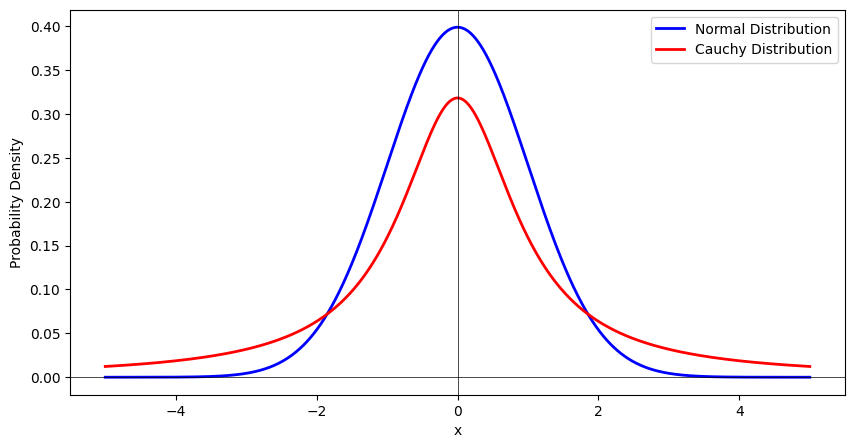
\includegraphics[width=0.9\linewidth]{Gaussian_Cauchy.png}
    \end{center}
\end{figure}

\subsection{The Loss Function}
The goal of the algorithm is now to get the similarities $P$ and $Q$ to be as close to each other as possible. 
A common choice for measuring the distance between two distributions is the Kullback-Leibler divergence. 

\begin{defi}[Kullback-Leibler Divergence]
    The \emph{Kullback-Leibler divergence} between two probability distributions $P$ and $Q$ over the same probability space is defined as:
    \[
    D_{\text{KL}}(P \parallel Q) = \sum_{x \in \mathcal{X}} P(x) \log\frac{P(x)}{Q(x)}
    \]
    for discrete distributions where \(\mathcal{X}\) is the domain of the distributions.
\end{defi}

The t-SNE algorithm now aims to find a low-dimensional representation $\mathcal{Y} = (y_1, \dots, y_n)$ that minimizes the KL-divergence between the similarity matrices $P$ and $Q$. 
We thus define the following loss function: 
\begin{equation}
    C(\mathcal{Y}) = D_{\text{KL}}(P \parallel Q) = \sum_{i,j \in \{1,\dots,n\}, i \neq j} p_{ij} \log \frac{p_{ij}}{q_{ij}}
\end{equation}
which leads to the following optimization problem: 
\begin{equation}
    (y_1, \dots y_n) = \argmin_{y_1, \dots y_n} C(\mathcal{Y}) = \argmin_{y_1, \dots y_n} \sum_{i,j \in \{1,\dots,n\}, i \neq j} p_{ij} \log \frac{p_{ij}}{q_{ij}}.
\end{equation}


Note that the Kullback-Leibler divergence is in fact not a metric, since it is not symmetric. 
One can observe that a large $p_{ij}$ being modeled by a small $q_{ij}$ leads to a bigger summand than using a large $q_{ij}$ to model a small $p_{ij}$. 
This means that our loss function places a large cost on using far-apart points to model points that are close in the original dataset. 
On the other hand, there is only a small cost to model points that are actually far apart as nearby in the embedding. 
This shows that we can expect a bigger focus on the preservation of local structure and is important to keep in mind when interpreting t-SNE embeddings, see \cite{Wa16Distill}. 

\subsection{Gradient Descent to Minimize Loss}
Minimizing the cost function can be achieved using a standard gradient-descent type algorithm, with an updating equation of 
\begin{equation}
    y_i^{(k+1)} = y_i^{(k)} + h \frac{\partial C}{\partial y_i}^{(k)} + m^{(k+1)}(y_i^{(k)} - y_i^{(k-1)}) 
\end{equation}
for $i=1,\dots,n$, where $h >0$ is a prespecified step size parameter, $m^{(k)} > 0$ is a momentum parameter and we denote the gradient of our loss function (with respect to $y_i$) as: 
%\begin{equation}
  %  \frac{\partial C}{\partial y_i}^{(k)} = 4 \sum_{1 \leq j \leq n, j \neq i} (y_j^{(k)} - y_i^{(k)}) S_{ij}^{(k)} \in \mathbb{R}^2 \text{ with } S_{ij}^{(k)} = \frac{p_{ij} - q_{ij}^{(k)}}{1+ \norm{y_i^{(k)}-y_j^{(k)}}_2^2 } \in \mathbb{R}
%\end{equation}
\begin{equation}
    \frac{\partial C}{\partial y_i}^{(k)} = 4 \sum_{1 \leq j \leq n, j \neq i} (p_{ij} - q_{ij}^{(k)}) q_{ij}^{(k)} Z^{(k)} (y_j^{(k)} - y_i^{(k)})
\end{equation}
where $Z$ is a global normalization constant: 
\begin{equation}
    Z^{(k)} = \sum_{m \neq l} (1 + \norm{y_m^{(k)} - y_l^{(k)}})^{-1}. 
\end{equation}
\textcolor{red}{\textbf{TO DO}: Check the gradient here, I'm pretty sure it should be $(y_i - y_j)$ and not the other way around}


% algorithm pseudocode here
\begin{algorithm}[H]
    \caption{Basic version of t-Distributed Stochastic Neighbor Embedding}
    \label{alg:tsne}
    \KwIn{data set $\mathcal{X} = \{x_1, x_2, \dots, x_n\}$, perplexity $\text{Perp}$, number of iterations $T$, learning rate $\eta$, momentum $\alpha(t)$}
    \KwOut{Low-dimensional representation $\mathcal{Y}^{(T)} = \{y_1, y_2, \dots, y_n\}$}


    Compute $p_{ij}$ with perplexity $\text{Perp}$ \;
    Sample initial solution $\mathcal{Y}^{(0)} = \{y_1, y_2, \dots, y_n\} \sim \mathcal{N}(0, 10^{-4} I)$\

    \For{$t = 1$ \KwTo $T$}{
        Compute low-dimensional affinities $q_{ij}$ \;
        Compute gradient $\frac{\delta C}{\delta \mathcal{Y}}$ \;
        Update solution:\;
        \[
        \mathcal{Y}^{(t)} = \mathcal{Y}^{(t-1)} + \eta \frac{\delta C}{\delta \mathcal{Y}} + \alpha(t) (\mathcal{Y}^{(t-1)} - \mathcal{Y}^{(t-2)})
        \]
    }

    \Return $\mathcal{Y}^{(T)}$\
\end{algorithm}
\textcolor{red}{\textbf{TO DO}: make algorithm look nicer}

To optimize the gradient descent prodcedure, \cite{vdMaa08} proposes the following: 
\begin{itemize}
    \item setting the momentum term to $\alpha^{(t)} = 0.5$ for $t<250$ and $\alpha^{(t)} = 0.8$ for $t \geq 250$
    \item set intial learning rate to $\eta = 100$ and update after every iteration adaptively using the adaptive learning rate scheme described by Jacobs \cite{Jacobs1988}
\end{itemize}



\section{Initialization}
here talk about pca init vs random one 
...
\section{Perplexity}
Let us come back to the variance $\sigma_i$ of the Gaussian centered at each datapoint $x_i$. What is a good value to choose? 
If we fixed a single value $\sigma$ to be the same for every datapoint, this is likely not a good choice, because real-life data often does not have a constant density everywhere but instead has sparser and denser regions. 
Given that we want to consider approximately the same number of nearest neighbors for each $x_i$, we opt to choose larger values of $\sigma_i$ for sparse regions and smaller bandwidths for dense regions. 

\textcolor{red}{\textbf{TO DO}: find a better way to describe what perplexity actually does, the following is just taken directly from \cite{vdMaa08}}

Any particular value of $\sigma_i$ induces a probability distribution $P_i$ over all other datapoints. 
The entropy of this distribution increases as $\sigma_i$ increases. 
The user can specify a specific so-called perplexity
\begin{equation}
    \kappa = \text{Perp}(P_i) = 2^{H(P_i)} 
\end{equation}
where $H(P_i) = -\sum_{j} p_{ij} \log_2 p_{ij}$ denotes the Shannon entropy of $P_i$. 

\textcolor{red}{\textbf{TO DO}: do we use $p_{ij}$ or $p_{j|i}$ in the definition of perplexity?}

Then, t-SNE performs a binary search for the value of $\sigma_i$ that produces the user-specified perplexity. 

One can think of perplexity as a smooth measure of the effective \textcolor{red}{\textbf{TO DO}: what does this actually mean?} number of neighbors being considered in the calculation of the $p_{ij}$. As such, larger perplexity values are computationally more expensive. 

\cleardoublepage        % Kapitel immer rechts beginnen
\chapter{Theoretical Results}\label{chapter:theoretical_results}
in which we give an overview of the theoretical work done on t-SNE so far. 
we will look at results from \cite{JMLR:v23:21-0524} and \cite{LinStei22}

\cleardoublepage        % Kapitel immer rechts beginnen
\chapter{Experiments}\label{chapter:experiments}

\section{Datasets}
We use the following datasets for our experiments (as well as synthetic data). 
\begin{itemize}
    \item Iris dataset \cite{iris_dataset}
    \item MNIST \cite{mnist_dataset}
    \item EMNIST letters \cite{emnist_dataset}
    \item flow cytometry \cite{flow_dataset}
    \item Macasko mouse retina \cite{Macosko_dataset} 
\end{itemize}

\section{Dataset Cluster Assumptions}
Here we investigate if assumptions made for clustering results in \cite{LinStei22} hold in practice, by looking at the simple Iris dataset. 
The reason that we look at Iris is that it is a very small dataset, which makes it feasible to look at all $N^2 = 150^2$ affinities $p_{ij}$ individually.  

Recalling \ref{eq:4.1}, we make the assumption that the data we perform t-SNE on is clustered. 
A natural question to ask then is: does real-life data that looks clustered to us humans fulfill this definition of clustered that is required: 
\begin{equation}
    p_{ij} \geq \frac{1}{10 N |\Omega(i)|}
\end{equation}
for all pairs of points $x_i, x_j$ that lie in the same cluster $\Omega(i)$? 

In order to investigate this question, we chose the Iris dataset. 
Ordering the data points in terms of cluster membership (there are 50 points of each of the three clusters), we can visualize what the high-dimensional similarity values $p_{ij}$ look like when using the standard parameters (perplexity = 30). 

\begin{figure}[h]
    %\begin{center}
    \centering 
        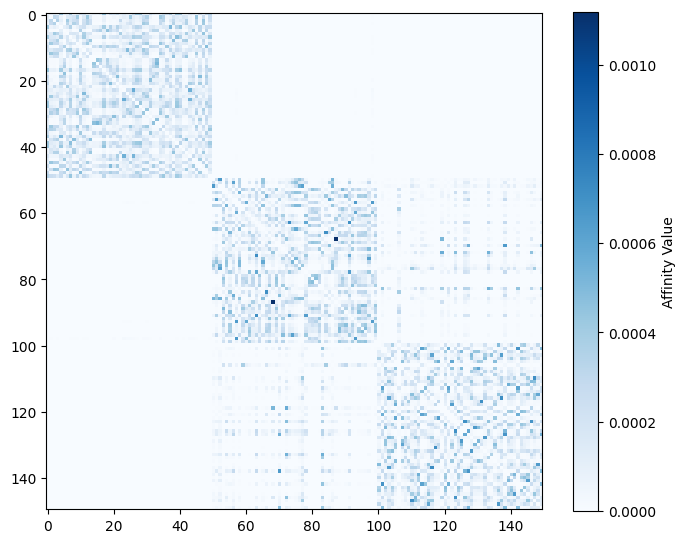
\includegraphics[width=0.7\linewidth]{figures/iris_affinity_matrix.png}
        \caption{Affinity values $p_{ij}$ of the Iris dataset visualized. The affinity matrix was generated using the standard perplexity value of 30.}
    %\end{center}
    \label{fig:iris_affinities}
\end{figure}

We can see the three clusters of the Iris dataset pretty clearly. 
From the visualization \ref{fig:iris_affinities}, it also seems like the first cluster is more well-defined than the second and third are. 
\textcolor{red}{If we run a dimensionality algorithm like PCA or t-SNE on it, we can also see that it performs well and clearly separates at least the first cluster from the other two.} 

So, it would seem that at least this first cluster would fulfil the condition that \begin{equation} p_{ij} \geq \frac{1}{10 N |\Omega(i)|} = \frac{1}{10 \cdot 150 \cdot 50} \end{equation}

However, when we investigate the $p_{ij}$ values of the first cluster (excluding, of course, the diagonal elements, since they are always zero), we notice that the smallest $p_{ij}$ value we observe is (rounded) $2.8 \cdot 10^{-7}$, whereas we calculated a lower bound of about $1.3 \cdot 10^{-5}$ above.
Furthermore, we calculated that a total number of 354 similarites between points in this same first cluster are smaller than the minimal $p_{ij}$ value required for it to be a cluster. 
Now, while \cite{LinStei22} do mention that there is some flexibility with respect to the exact constant being used - we would have to increase it by two orders of magnitude for this result to hold. 

For the last two clusters, we observe something even more interesting. 
If we consider the second cluster, we see that that the smallest similarity value between two points in it is $0.0$. 
This makes it virtually impossible to consider as a cluster, not matter how far we would scale the constant. 
One might argue that indeed clusters 2 and 3 belong together, but also then we observe some points having $0$ similarity to each other. 

\section{Initialization}
Here we reproduce results from \cite{kobak21} on synthetic data and show that t-SNE with PCA initialization can reconstruct geometric shapes up to some extent. 

We also investigate the effects of PCA initialization on real-world datasets. 

\section{An Implementation of Rescaled t-SNE for Large Data Limits}
something here 

\section{Effect of Varying Perplexity Values}
there were some figures here before I removed them. 

\section{Early Exaggeration}
what effect does it have? 

\section{opt-SNE Implementation}
and comparison to default settings 

%\cleardoublepage
%\appendix
\chapter*{Appendix}
\addcontentsline{toc}{chapter}{Appendix}
\renewcommand{\thesection}{\Alph{section}}
\section{a}
\section{b}

% Weitere Symbole für das Symbolverzeichnis
\symbolindex[f]{$F$}{A topological or Riemann surface.}{}

% Symbolverzeichnis
\cleardoublepage        % Auch diese sollen auf der rechten Seite beginnen
\printnomenclature      % Symbolverzeichnis ausgeben

% Stichwortverzeichnis
\cleardoublepage        % Auch diese sollen auf der rechten Seite beginnen
\printindex             % Stichwortverzeichnis ausgeben

% Referenzen
\nocite{*}              % Alle Einträge der Bib-Datei sollen in die Referenzen
\cleardoublepage        % Auch diese sollen auf der rechten Seite beginnen
\printbibliography      % Bibliographie ausgeben.

\end{document}